% Anna og Sune (3.2)

%TODO:
% Introduction to data collection, data processing and closing the sensing loop


\section{Data Collection}
% TODO: 
% Apply definitions
% Little introduction
% Tactics:
%    - Part into intervals
%    - Sampling rate
%    - Combinations of sensors (location/gps + 
%      accelerometer + gyroscope)
% Relate to articles
% Relate to app
% Reflect and discuss

The first part of continuous sensing is the data collection. In this section the data collection process of our application will be described along with ideas for extension.
Data collection needs to deal with the concepts of sensor choice, sampling rate and phone context, which can be determined using a tactic of a defined quality attribute. When developing on a mobile device the energy efficiency tactics will most likely be applied, since the battery life is a very valuable asset.  

The data collection from continuous sensing in our application consists of: 
\begin{itemize}
    \item Location data - GPS sensor (Fine Location)
    \item Activity Recognition data from Google API - Low-power Sensors \cite{androidActivity}
\end{itemize}

Location data uses the fine location sensor to determine the actual path of the bike route when a bikebus has startet. To determine when a bikebus has startet and ended the notion of "Geofencing" is used to trigger when the user is inside a radius of \textcolor{red}{<<INSERT RADIUS>>}. 
When a geofence event has been raised some constraints must be fulfilled before the continuous data collection can begin.
\begin{itemize}
    \item The current timestamp must be within the time window textcolor{red}{<<INSERT TIME WINDOW>>} of an enlisted bikebus
    \item The current activity must be of type "ON\_BICYCLE"
\end{itemize}
Once the constraints have been fulfilled the data collection begins \textcolor{red}{<<INSERT SENSING TACTIC>>} by collecting locations at the sample rate of \textcolor{red}{<<INSERT SAMPLE RATE>>}. This is fairly expensive sensor collection because the fine location sensor is used to give street-specific accuracy of the location data. This expensive sensing operation can be improved by decreasing the sample rate (\textcolor{red}{<<SPECIFY EXACTLY WHICH TACTICS THIS IS>>}) and afterwards apply some filtering techniques to smooth out the path.

Along with the location data the data collection also includes Activity Recognition for assuring all collected data only is collected while biking. This eliminates the situations where stopping for a red light is accounted for in the data collection and therefore will influence the overall statistics. This combination of location and activity data will provide more accurate biking statistics. 
The activity recognition only uses the sensors defined as "Low-power".
According to the Android documentation of "Low-power sensors" \cite{androidLow} the following sensors can be utilized:
\begin{itemize}
    \item Geomagnetic rotation vector
    \item Significant motion
    \item Step counter
    \item Step detector
    \item Tilt detector
\end{itemize}
The use of only "Low-power sensors" makes the activity recognition relatively energy efficient opposed to the location data.

Once the end geofence event arises the data collection can stop and the final statistics will be processed. Due to the incident of the end geofence never being triggered due to inaccurate location sensing, the program automatically stops the data collection if the current time exceeds a given time threshold \textcolor{red}{<<INSERT TIME THRESHOLD>>} defined from the suggested time duration of the current bikebus.

\section{Data Processing}
% TODO:
% Apply definitions
% Little introduction
% Explain Types of processing
%    - online/offline processing
%    - realtime/batch processing
% Explain processing math
%    - classification (basic)
%    - filtering algorithms
%    - compression algorithms (Trajection)
% Relate to articles
% Relate to app
% Reflect and discuss

When working with location based data one needs to take into account the amount of data which need to be processed and stored. Figure \ref{fig:system_model_for_locations_based_services} from \cite{Lee2011} shows how moving objects gathers data and sends it to mobile object databases. The location server will then be able to serve different kinds of locations based application. The leads to how Bikebus can be designed only to store the most valuable data without losing precision of data. Bikebus has cases were it could be beneficial to visualize route data or do statistical calculation on the route data.   

\begin{figure}[H]
\centering
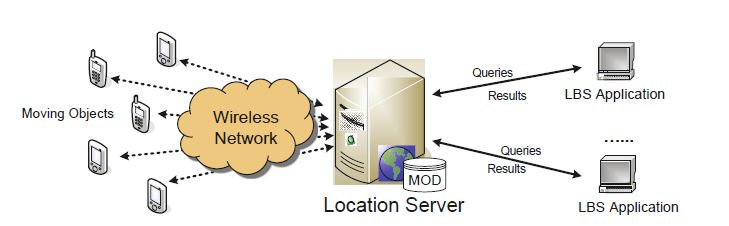
\includegraphics[scale=0.6]{LocationServer.JPG}

\caption{System model for locations based services}
\label{fig:system_model_for_locations_based_services}
\end{figure}


There are several options presented by \cite{Lee2011} how one can do data reduction and filtering techniques on spatial trajectories and thereby reduce the amount of data saved. There is batch compression (offline) and online algorithms for data reduction. Batch compression do computation on a full set of location points and then transmits it to the location server. Online algorithms computes directly on online selective data. We have created prototypes  of an offline and online algorithm namely Douglas-Peucker (DP) and Sliding Window. The implementations are elaborated in section~\ref{sec:prototypes}. 

Figure \ref{fig:douglas_peucker_algorithm} illustrates how DP using perpendicular Euclidian distance as the error measure together with a approximated trajectory (dotted line) and the original trajectory. If the error measure doesn't meet the threshold ($p_9$) a split point is created at ($p_9$). This results in a trajectory $p_0,p_9,p_{16}$. This process is repeated until the error measure between the approximated trajectory and the original trajectory is below the error threshold. The algorithm proceeds until all the location points in the original trajectory are visited.   

\begin{figure}[H]
\centering
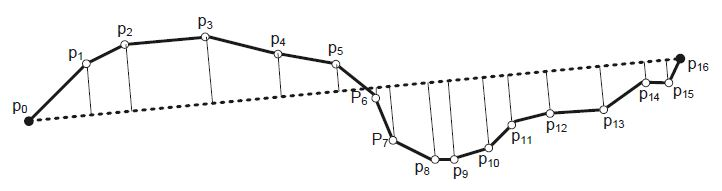
\includegraphics[scale=0.6]{DP.JPG}
\caption{Douglas-Peucker offline algorithm}
\label{fig:douglas_peucker_algorithm}
\end{figure}


The idea behind sliding window is to fit locations points in a growing sliding window with a valid line segment. The window continue to grow until approximation error threshold exceeds. The algorithm initializes the first location point of a trajectory as the anchor point $p_a$ of the window. The window slides when a new location point $p_i$ is added. As long all points within the sliding window doesn't exceeds the error threshold against a line segment new points are added. If the error threshold is violated the $p_{i-1}$ is included as part of the approximated trajectory and the $p_i$ is set to be the new anchor point $p_a$. An example of the sliding window is illustrated in figure \ref{fig:sliding_window_algorithm}. First the anchor point is set to $p_0$. The window slides \{$p_0,p_1,p_2,p_3,p_4$\} until $p_4$ is processed. Because the error threshold is violated for some location point within the sliding window, $p_3$ is included as a part of the approximated trajectory. The new anchor point $p_a$ is set to $p_3$.       
\begin{figure}[H]
\centering
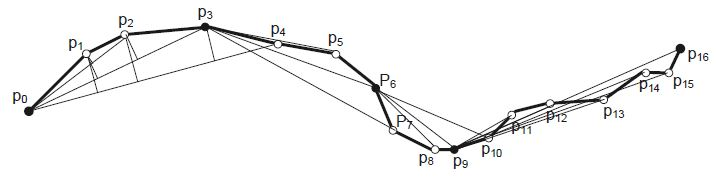
\includegraphics[scale=0.6]{SlidingWindow.JPG}

\caption{Sliding Window online algorithm}
\label{fig:sliding_window_algorithm}
\end{figure}


An alternative to sliding window is the open window algorithm. It is similar to the sliding window excepts when the error threshold is violated. The algorithm chooses the location point with the largest error distance as a part of the approximate trajectory whereas the sliding window included $p_{i-1}$ location point. This algorithm result in more accuracy compared to sliding window. 

\begin{figure}[H]
\centering
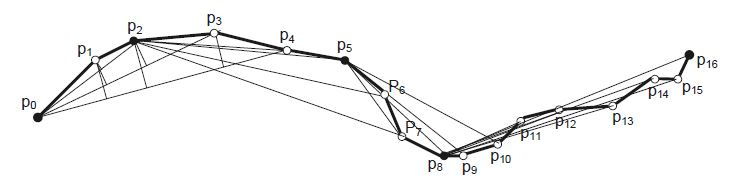
\includegraphics[scale=0.6]{OpenWindow.JPG}

\caption{Open Window online algorithm}
\label{fig:open_window_algorithm}
\end{figure}

These compressions algorithms suffers under location points which are potentially outliers. The compression isn't able to distinguish between "good" and "bad" points. One way to handle this is by applying a median filter. 

\iffalse
Suggestions for further processing:
\begin{itemize}
    \item Median filtering
    \item Advanced statistics calculations (analyse per interval)
    \item Algorithm to balance the trade-off between processing space and time (Appendix \ref{app:processing_algorithm})
\end{itemize}
\fi

\section{Closing the Sensing Loop}
% TODO:
% Apply definitions
% Little introduction
% Explain concepts
%    - Sharing
%    - Privacy 
%    - Personalization
% Relate to articles
% Relate to app: 
%    - privacy: delete raw data after processing
% Reflect and discuss
Closing the sensing loop deals with the final step of the continuous sensing where the collected and processed data is used to create value for the end user.
This is typically done by sharing the data either individually, with a group or for the community. 
Closing the sensing loop in our application happens after a bikebus has finished, where the data collection stops and the data is processed. Currently the newly processed statistics are added to the personal statistics for each user. These statistics will present the development of the user's cycling statistics.

Another idea for closing the sensing loop is to share the data with the municipality to gain better insight in people's cycling routines. This can benefit the community by detecting bottlenecks on bike paths (i.e. caused by poor traffic lighting or poor road construction) or missing bike parking in the city etc. 
The current application with individual sensing now becomes community sensing based instead.

When expanding the data sharing to the community the issue of privacy needs to be addressed. Location coordinates can be very sensitive private data and should be anonymous before sharing with the community.  

Ideas for applying privacy:
\begin{itemize}
    \item Share only the location and timestamp data and let the server assign the data a auto-generated primary key for the database. This makes all data independent from each other and the user.
    \item Share the data as batch file once a day to minimize live monitoring each user. Even though the location data is not connected to a specific person, it can be invasive to know that a person is at a specific place at the given moment.
\end{itemize}

In the article \cite{Mun2009} three different privacy countermeasures have been identified, which might be helpful to create more anonymous location data:
\begin{itemize}
    \item Selective Hiding: Generate location traces based on historical data to hide the actual data
    \item Spatial Routing: Use more coarse location data to blur out the fine location data
    \item Noise Addition: There is generated some noise of a location coordinate based on statistical distributions to be added to the coordinate
\end{itemize}

Of course there is a trade-off between the privacy and accuracy of the location data, which may be adjusted according the size of privacy needs and location accuracy. For instance when monitoring traffic data, the countermeasures should still be able to show which roads are used, else the data is not beneficial for traffic analysis.
